%% =====================================================================
%% Phase 2 Report — ACM sigconf (acmart) template
%% Course: AI in Healthcare (High-Risk Project), UT Austin, Summer 2026
%%
%% HOW TO COMPILE
%%   Easiest: upload this .tex and the figures/ folder to a new Overleaf
%%   project (overleaf.com). Overleaf ships acmart; it compiles as-is with
%%   pdfLaTeX. No .bib file is needed — references are inline below.
%%
%% NOTE: [nonacm] drops the ACM copyright strip, which is correct for a
%% course paper. Remove it only if you are submitting to an actual ACM venue.
%% =====================================================================
\documentclass[sigconf,nonacm]{acmart}

\usepackage{booktabs}
\usepackage{graphicx}
\graphicspath{{figures/}}

%% Silence ACM boilerplate that does not apply to a course submission.
\settopmatter{printacmref=false}
\renewcommand\footnotetextcopyrightpermission[1]{}
\pagestyle{plain}

\begin{document}

\title{Unlocking Latent Clinical Knowledge with Parameter-Efficient
Fine-Tuning}
\subtitle{A QLoRA Approach to In-Hospital Mortality Prediction on
Constrained Hardware}

\author{Thomas I. Bales}
\affiliation{%
  \institution{The University of Texas at Austin}
  \department{AI in Healthcare (High-Risk Project)}
  \city{Austin}\state{Texas}\country{USA}
}
\email{tibales@utexas.edu}

\renewcommand{\shortauthors}{Bales}

\begin{abstract}
Early identification of ICU patients at high risk of in-hospital mortality
supports triage and timely intervention, but deploying predictive models in
care settings demands more than raw accuracy: it demands reproducibility,
auditability, and an honest account of cost. We ask whether a small, open
foundation model---\texttt{llama-3.1-8B}---can be made to \emph{beat its own
untuned self} on a specialized clinical task using a parameter-efficient
adapter of only 6.8M trainable parameters (0.08\% of the model), trained end
to end on a single 16\,GB GPU. Using patient descriptions derived from
MIMIC-III and 4-bit QLoRA fine-tuning, and after finding and removing a
critical validation-set leak, the adapted model improves held-out recall from
0.18 to 0.46, precision from 0.11 to 0.56, and accuracy from 74.5\% to 90.0\%
on 200 patients never seen during training---gains on both axes at once. We
characterize the recall--precision oscillation observed during training as a
clinical-\emph{values} decision rather than a technical default, trace the
performance ceiling to conflicting labels in coarse features, and argue that
deterministic (temperature 0.0) inference is a prerequisite for clinical
auditability. All results were produced at near-zero marginal energy cost,
foregrounding a governance question about where the energy of this capability
was actually spent.
\end{abstract}

\begin{CCSXML}
<ccs2012>
<concept><concept_id>10010147.10010257</concept_id>
<concept_desc>Computing methodologies~Machine learning</concept_desc>
<concept_significance>500</concept_significance></concept>
<concept><concept_id>10010405.10010481</concept_id>
<concept_desc>Applied computing~Health informatics</concept_desc>
<concept_significance>500</concept_significance></concept>
</ccs2012>
\end{CCSXML}
\ccsdesc[500]{Computing methodologies~Machine learning}
\ccsdesc[500]{Applied computing~Health informatics}

\keywords{clinical NLP, mortality prediction, LoRA, QLoRA, parameter-efficient
fine-tuning, MIMIC-III, model governance, AI in healthcare}

\maketitle

%% =====================================================================
\section{Introduction}
%% =====================================================================
In-hospital mortality is one of the oldest and most consequential prediction
targets in critical care. A model that flags, early in an admission, which
patients are at elevated risk of dying can inform triage, prompt escalation of
care, and focus scarce clinician attention where it matters most. Because a
missed death is far costlier than a false alarm, the metric that matters is
not overall accuracy but \emph{recall}---and recall is precisely what a naive
classifier sacrifices, since at an 11\% base rate a model that predicts
``survives'' for everyone already scores 89\% accuracy while catching nobody.

Two forces make this an interesting problem in 2026 rather than a solved one.
First, open foundation models such as \texttt{llama-3.1-8B}~\cite{llama3} now
encode a great deal of latent clinical knowledge absorbed during pretraining.
Second, parameter-efficient fine-tuning (PEFT)~\cite{lora,qlora} makes it
possible to adapt such a model with a tiny fraction of its parameters, on
hardware a research group or a hospital IT department already owns. The
natural question---and the ``high-risk'' bet of this project---is whether a
small, general, open model can be made to \emph{outperform its own zero-shot
baseline} on a specialized clinical task, using an adapter that trains in a few
hours on a single GPU, and whether the result can be made reproducible and
auditable enough to be defensible in a care setting.

This framing is deliberately about more than a leaderboard number. Deploying a
predictive model in healthcare raises three questions that a benchmark hides:
(i) \emph{at what operating point} should the model run, given that catching
more deaths always means more false alarms; (ii) \emph{what is the model
actually learning}, and where does the data stop it; and (iii) \emph{what did
the capability cost}, and who paid for it. We treat these not as afterthoughts
but as first-class results.

\paragraph{Contributions.} This paper reports:
(1) an end-to-end QLoRA fine-tuning pipeline for mortality prediction that runs
on a single 16\,GB GPU;
(2) a rigorous held-out evaluation made trustworthy only after discovering and
removing a validation-set leak that would have invalidated the headline claim;
(3) a characterization of the recall--precision operating frontier as a
clinical-values decision;
(4) identification of a data-resolution ceiling caused by conflicting labels in
coarse features; and
(5) an honest account of the memory and thermal constraints that dominated the
engineering effort.

%% =====================================================================
\section{Related Work}
%% =====================================================================
\paragraph{Parameter-efficient fine-tuning.}
LoRA~\cite{lora} freezes a pretrained model and injects trainable low-rank
matrices into its attention projections, cutting the number of trainable
parameters by orders of magnitude while matching full fine-tuning quality on
many tasks. QLoRA~\cite{qlora} extends this by quantizing the frozen base model
to 4 bits (NF4) and back-propagating through it, enabling fine-tuning of models
that would not otherwise fit in a single GPU's memory. Both works address the
same obstacle this project faced---adapting a large model under a hard memory
budget---and our method is a direct application of their techniques to a
clinical setting.

\paragraph{Language models for clinical prediction.}
Rasmy et al.'s Med-BERT~\cite{medbert} pretrains a transformer on structured
diagnosis codes from large EHR corpora and shows gains on downstream disease
prediction, establishing that clinical-domain pretraining transfers to
prediction tasks. Jiang et al.~\cite{nyutron} scale this idea to a
health-system deployment (NYUTron), fine-tuning a language model on unstructured
clinical notes to predict outcomes including in-hospital mortality and
readmission, and report performance competitive with structured models. Both
rely on large-scale clinical pretraining or health-system-scale infrastructure.
Our work asks a complementary question: how far can a \emph{small, general,
open} model plus a 0.08\% adapter get on commodity hardware, and it foregrounds
the governance dimensions those deployment-focused papers necessarily treat as
secondary.

\paragraph{Data foundation.}
All patient records derive from MIMIC-III~\cite{mimic3}, a de-identified
critical-care database that has become a standard benchmark substrate for
clinical machine learning. We use a coarse, 17-feature view of each admission
(see Section~\ref{sec:method}), which---as we show---is both the source of the
model's efficiency and the source of its ceiling.

%% =====================================================================
\section{Methodology}\label{sec:method}
%% =====================================================================
Figure~\ref{fig:workflow} summarizes the end-to-end workflow, from raw MIMIC-III
admissions through data auditing to held-out evaluation. We describe each stage
below.

\begin{figure*}[t]
  \centering
  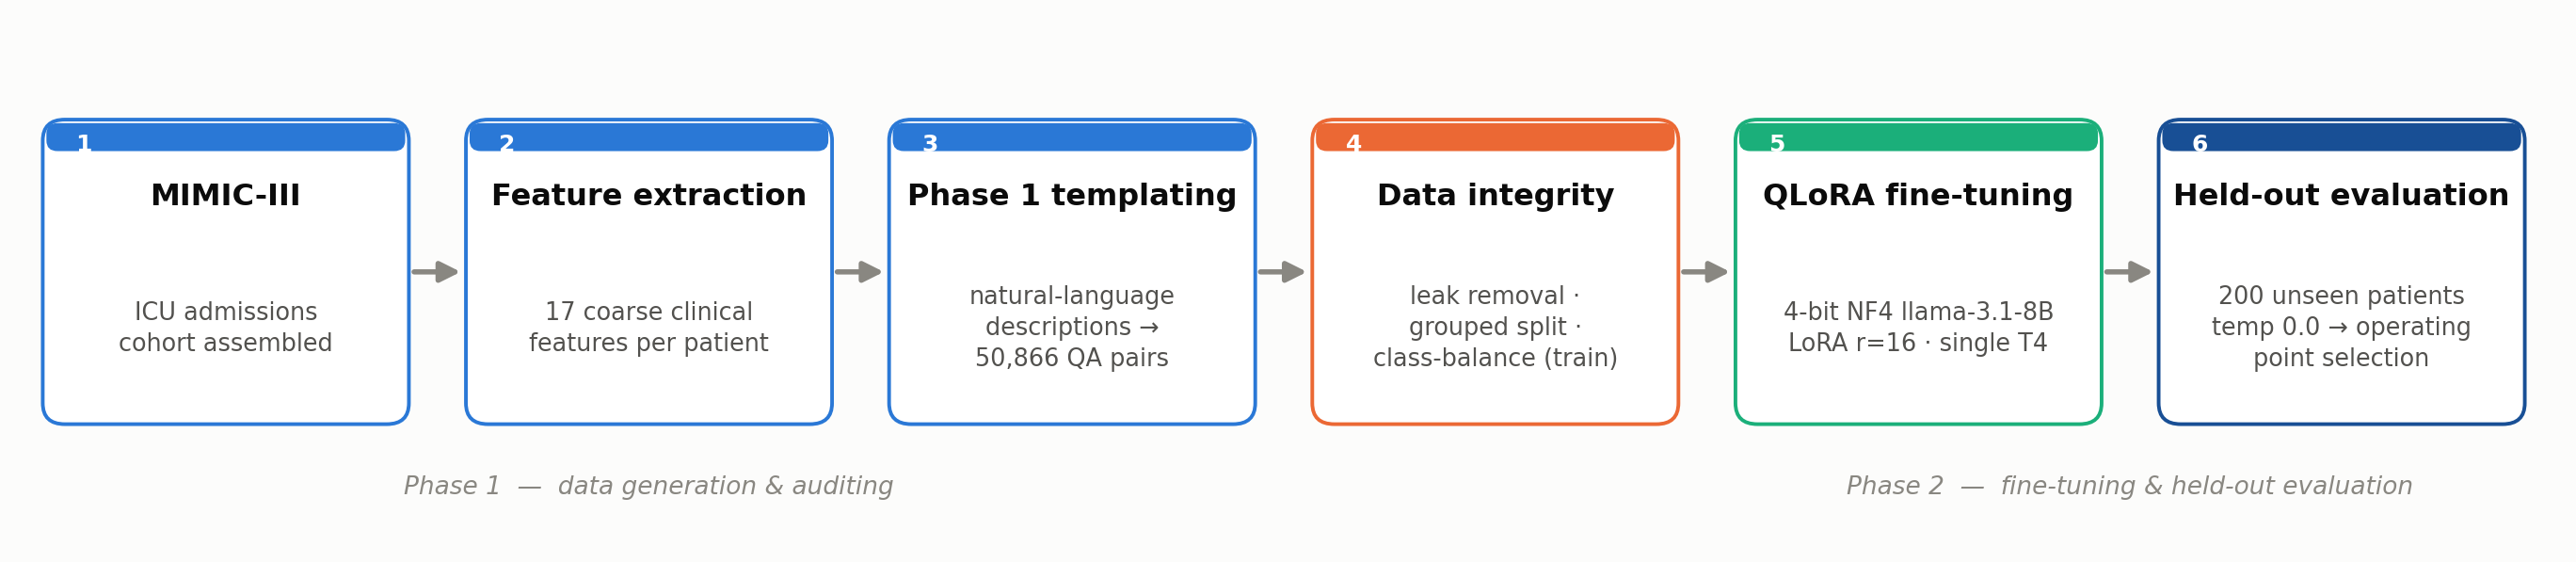
\includegraphics[width=\textwidth]{workflow.png}
  \caption{End-to-end workflow. Phase 1 assembles a cohort from MIMIC-III,
  reduces each admission to 17 coarse features, and templates it into a
  natural-language description with a one-token \texttt{Yes}/\texttt{No}
  mortality answer (50{,}866 pairs). Phase 2 audits the data for leakage and
  label conflicts, fine-tunes a 4-bit \texttt{llama-3.1-8B} with a LoRA adapter
  on a single T4 GPU, and evaluates on 200 held-out patients at temperature
  0.0. The orange stage (data integrity) is where the most consequential
  correction was made.}
  \label{fig:workflow}
\end{figure*}

\subsection{Data and cohort}
Each ICU admission in the cohort is reduced to 17 coarse clinical features
(e.g., age band, gender, insurance/payer, length of stay, diagnosis count,
substance-use flags). A templating step (Phase 1) renders each admission as a
short natural-language description paired with an instruction and a single-token
answer---\texttt{Yes} or \texttt{No} for in-hospital mortality---using eight
distinct instruction templates. The resulting corpus contains 50{,}866
instruction--answer pairs over 49{,}377 distinct descriptions, with a class
balance of 11.4\% positive (deaths).

\subsection{Data integrity}
Two problems, invisible from the model's loss curve, were found by inspecting
the Phase 1 output directly.

\emph{Validation leakage (critical).} All 200 patient descriptions in the
held-out validation sample also appeared, verbatim, in the training corpus. As
originally written, the pipeline would have trained on those patients and then
reported ``validation accuracy'' on the same patients, comparing it against a
zero-shot baseline that had never seen them---measuring memorization, not
generalization, and invalidating the headline comparison. We exclude those
patients from training (213 pairs dropped) and verify that 0 of 200 remain in
either the training or evaluation split.

\emph{Conflicting labels (a data ceiling).} 265 descriptions carry \emph{both}
\texttt{Yes} and \texttt{No} labels: because the 17 features are coarse,
distinct admissions with different outcomes render identical text. No amount of
training can separate contradictory examples, so this sets an irreducible noise
floor on achievable accuracy.

\emph{Honest splitting.} Because 1{,}300 descriptions appear in multiple pairs,
we split by description (a grouped split), not at random, yielding 48{,}653
training and 2{,}000 evaluation pairs with zero description overlap. Crucially,
we rebalance \emph{only} the training split (majority-to-minority ratio 2.0);
the evaluation split retains natural prevalence (12\% positive), so that
evaluation precision is not inflated and agrees with the final 200-patient
validation.

\subsection{Model and quantization}
The base model is \texttt{llama-3.1-8B} (8.03B parameters). In fp16 it requires
$\approx$16.1\,GB, exceeding the 15.9\,GB of the target GPU before optimizer
state or activations. We therefore load it in 4-bit NF4 with double
quantization and fp16 compute (the Turing-class GPU has no bf16), reducing the
footprint to 5.6\,GB. A LoRA adapter (rank 16, $\alpha$=32, dropout 0.05) is
attached to the query and value projections, giving 6{,}815{,}744 trainable
parameters---0.08\% of the model. The base weights stay frozen; only the
adapter is trained.

\subsection{Training}
We train for one epoch with an effective batch size of 8 (micro-batch 4,
gradient accumulation 2), learning rate $2\times10^{-4}$ with 100 warmup steps,
and gradient checkpointing. Sequences are capped at 128 tokens with dynamic
per-batch padding (measured median length 97), and prompt tokens are masked to
$-100$ so the loss is computed on the answer token alone---a change that
concentrates the gradient on the prediction rather than on regurgitating
boilerplate. We monitor a held-out eval split every 150 steps on
accuracy, recall, precision, and F1, and keep the best checkpoint by F1.

\subsection{Evaluation protocol}
Final evaluation uses a 200-patient sample held out entirely from training. We
compare the untuned base model at zero-shot against the same base with the LoRA
adapter, both decoded greedily at \textbf{temperature 0.0}. Determinism is not a
tuning preference here but a requirement: at temperature 0.0 the same patient
always yields the same assessment, which is what makes the system auditable.

\subsection{Systems constraints}
Two hardware realities shaped the design. \emph{Memory:} with checkpointing off,
batch $8\times2$ exceeded the GPU; the shipped configuration (batch $8\times2$,
checkpointing on) peaks at 10.73\,GB. \emph{Thermal:} the GPU is a passively
cooled 70\,W datacenter card that, in a desktop chassis, throttles roughly
$4\times$ within about 100 seconds of sustained load. A sequence of improvised
interventions---an air duct, a floor fan ($\approx$\$30), a 60\,W power cap, and
a batch-size reduction---held it at a stable 94\,\textdegree C, about
2\,\textdegree C inside the hardware shutdown threshold, for the full run.

%% =====================================================================
\section{Results}
%% =====================================================================
\subsection{Held-out performance}
Table~\ref{tab:headline} and Figure~\ref{fig:bars} report the headline result on
the 200 held-out patients. The adapted model improves on the zero-shot base on
\emph{every} metric simultaneously: it catches 2.5$\times$ as many deaths and is
roughly 5$\times$ more precise when it does flag a patient. It did not trade one
axis for the other, and it did not collapse into the majority class.

\begin{table}[h]
  \caption{Held-out results on 200 patients never seen in training. Both models
  are the same \texttt{llama-3.1-8B}; only the 0.08\% adapter differs.}
  \label{tab:headline}
  \begin{tabular}{lccc}
    \toprule
    Metric & Zero-shot base & LoRA fine-tuned & Change \\
    \midrule
    Recall (deaths caught)   & 0.18 (4/22)  & \textbf{0.46 (10/22)} & 2.5$\times$ \\
    Precision (flags correct)& 0.11         & \textbf{0.56 (10/18)} & $\sim$5$\times$ \\
    Accuracy                 & 74.5\%       & \textbf{90.0\%}       & +15.5 pt \\
    Deaths flagged           & 4 of 22      & \textbf{10 of 22}     & +6 \\
    \bottomrule
  \end{tabular}
\end{table}

\begin{figure}[h]
  \centering
  
\includegraphics[width=\columnwidth]{zeroshot_vs_lora.png}
  \caption{Zero-shot base vs. LoRA fine-tuned on the same 200 held-out patients,
  both at temperature 0.0. Improvement is on both axes at once.}
  \label{fig:bars}
\end{figure}

\subsection{Confusion matrix}
Figure~\ref{fig:cm} shows the held-out confusion matrix for the adapted model. Of
22 true deaths it catches 10 (true positives) and misses 12; of 178 survivors it
false-alarms on only 8. The total number of patients flagged (18) sits near the
true death count (22), indicating that the model learned the correct
\emph{scale} of the problem---a calibrated, usable operating point rather than a
model that flags everyone or no one.

\begin{figure}[h]
  \centering
  
\includegraphics[width=0.92\columnwidth]{confusion_matrix.png}
  \caption{Held-out confusion matrix (LoRA). Color encodes each cell's share of
  its row so both rows remain legible despite the 170-vs-rest class imbalance.}
  \label{fig:cm}
\end{figure}

\subsection{Training dynamics as an operating frontier}
Across one epoch the run passed through four visible phases (from the run's
evaluation log): an initial \emph{collapse} (recall 0, hiding in the base
rate); a \emph{breakout} in which class-balanced training pulled the model off
the base rate and recall oscillated violently; a \emph{damping} phase as the
learning rate decayed; and \emph{convergence}, with F1 peaking and the flag
count settling near the true death count. The oscillation is itself a result. At
two adjacent steps the same weights presented opposite operating points---an
aggressive point (recall 0.51, precision 0.26, many flags) and a conservative
one (recall 0.15, precision 0.69, few flags). The model did not get better or
worse between them; it moved along its own recall--precision frontier.

\subsection{Efficiency}
The entire result was obtained by training 6.8M parameters (0.08\% of the
model), on a 5.6\,GB quantized base, on a single GPU, for an added hardware cost
of about \$30, with fully deterministic inference. The medical knowledge that
made it work was already frozen in the pretrained weights; fine-tuning
\emph{unlocked} it rather than adding it.

%% =====================================================================
\section{Discussion}
%% =====================================================================
\paragraph{The operating point is a values decision.}
Because the same weights can be read at many thresholds, choosing where to
operate---how many false alarms are acceptable to catch one more death---is not
a technical default to be chosen silently by a library. It is a clinical-values
decision that belongs to an accountable institution. Reporting a single number
hides exactly the choice that governance should own.

\paragraph{The ceiling is the data, not the model.}
The residual oscillation never fully vanished because the limit is in the
features: contradictory labels (Section~\ref{sec:method}) mean no decision
boundary can be stable. This points directly at the highest-value improvement:
richer features (raw labs, vital signs, diagnosis codes) that separate patients
the current descriptions collapse together. The bottleneck is feature
resolution, not model capacity or method.

\paragraph{A fairness note on proxies.}
Feature selection dropped race but retained insurance/payer. In the MIMIC
cohort, payer encodes race and class; a model that omits race but keeps its
proxy can appear fair on a checklist while distributing its errors along the
axis the omission was meant to protect. Whether to remove the proxy, keep and
flag it, or fund the intervention the disparity implies is a policy question,
not a technical one.

\paragraph{Energy was spent upstream.}
The large energy cost of this capability was front-loaded into pretraining,
absorbed by whoever trained the base model and inherited here for free.
Fine-tuning to beat that base cost near-zero marginal energy. That
asymmetry---ecological cost socialized upstream, benefit accruing to every
downstream fine-tuner---is itself a governance question about who authorized the
expenditure on behalf of everyone who now depends on it.

\paragraph{Limitations.}
The headline is a single 200-patient validation sample under one random seed;
confidence intervals at this size are wide. The step-level training dynamics
come from a single run's log rather than a saved artifact. MIMIC-III is a single
institution's historical data, so external validity is unestablished. We report
a discrimination operating point but not a calibration analysis.

%% =====================================================================
\section{Conclusion and Future Work}
%% =====================================================================
A small custom adapter on a small, open foundation model beat that model's own
zero-shot baseline on in-hospital mortality prediction---improving recall,
precision, and accuracy at once---at minimal compute and energy cost and with
deterministic, auditable output. Just as important as the numbers is the
discipline behind them: a validation leak that would have invalidated the claim
was found and removed, the performance ceiling was traced to the data rather
than the model, and the operating point was framed as the clinical-values
decision it is.

Future work follows directly. \emph{Feature enrichment}---replacing coarse
counts with raw labs, vitals, and diagnosis codes---is the single highest-value
step for lowering the conflicting-label noise floor. We would report the full
recall--precision frontier across checkpoints rather than a single point, run an
\emph{ensemble check} against structured baselines (gradient-boosted trees,
AUC~0.757; a deep network, AUC~0.754) to test whether the text model misses
\emph{different} patients, and add calibration and external validation. A
planned Phase 3 explores a retrieval-augmented, clinical-persona architecture as
a third comparison point. If redone, we would save per-step evaluation
artifacts from the outset and budget for adequate GPU cooling before, not
during, the run.

%% =====================================================================
\begin{thebibliography}{9}

\bibitem{lora}
E.~J. Hu, Y.~Shen, P.~Wallis, Z.~Allen-Zhu, Y.~Li, S.~Wang, L.~Wang, and
W.~Chen. 2022.
\newblock LoRA: Low-Rank Adaptation of Large Language Models.
\newblock In \emph{Int. Conf. on Learning Representations (ICLR)}.

\bibitem{qlora}
T.~Dettmers, A.~Pagnoni, A.~Holtzman, and L.~Zettlemoyer. 2023.
\newblock QLoRA: Efficient Finetuning of Quantized LLMs.
\newblock In \emph{Advances in Neural Information Processing Systems
(NeurIPS)}.

\bibitem{mimic3}
A.~E.~W. Johnson, T.~J. Pollard, L.~Shen, L.~H. Lehman, M.~Feng, M.~Ghassemi,
B.~Moody, P.~Szolovits, L.~A. Celi, and R.~G. Mark. 2016.
\newblock MIMIC-III, a freely accessible critical care database.
\newblock \emph{Scientific Data} 3, 160035.

\bibitem{nyutron}
L.~Y. Jiang, X.~C. Liu, N.~P. Nejatian, et al. 2023.
\newblock Health system-scale language models are all-purpose prediction
engines.
\newblock \emph{Nature} 619, 357--362.

\bibitem{medbert}
L.~Rasmy, Y.~Xiang, Z.~Xie, C.~Tao, and D.~Zhi. 2021.
\newblock Med-BERT: pretrained contextualized embeddings on large-scale
structured electronic health records for disease prediction.
\newblock \emph{npj Digital Medicine} 4, 86.

\bibitem{llama3}
A.~Grattafiori et al. (Llama Team, AI @ Meta). 2024.
\newblock The Llama 3 Herd of Models.
\newblock \emph{arXiv preprint} arXiv:2407.21783.

\end{thebibliography}

\end{document}
